W~pierwszej kolejno�ci zaj�li�my si� regulatorami liniowymi. Ze wzgl�du na baga� do�wiadcze� (oraz emocjonalny) nabyty w~ci�gu dw�ch lat regularnego obcowania z~obydwoma algorytmami, zdecydowali�my si� na dostrojenie ich \textbf{metod� in�yniersk�}. Jak pokaza�y dalsze testy, pozwoli�o nam to na uzyskanie lepszych efekt�w ni� w~przypadku wykorzystania gotowych algorytm�w optymalizacyjnych dost�pnych w~pakiecie \verb!optimisation toolbox!. 

\begin{figure}[H]
    \makebox[0.21\textwidth]{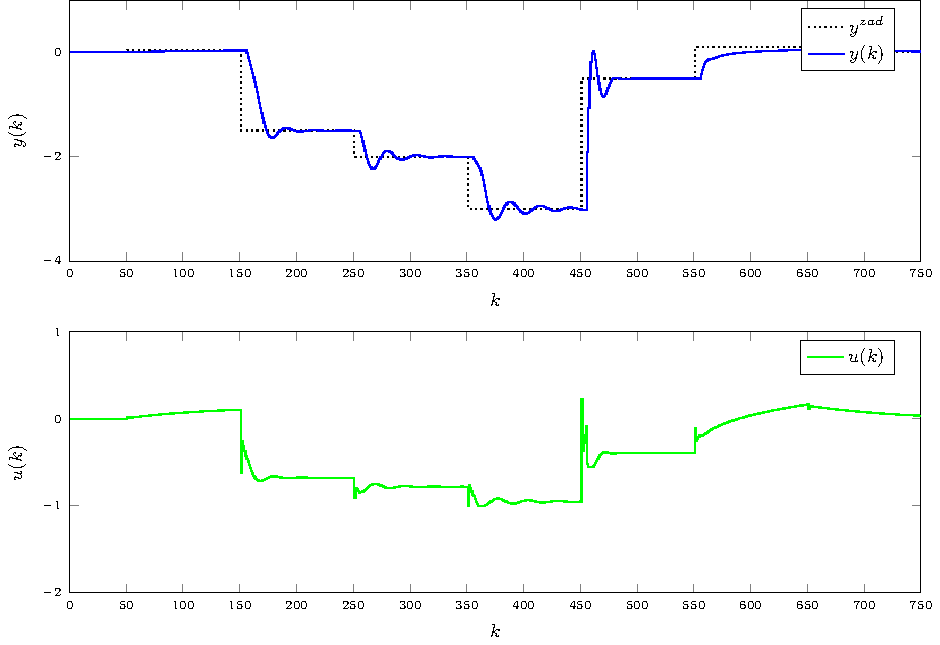
\includegraphics[width=0.2\paperwidth, height=0.15\paperheight]{data/Desired_plot_PID_number_of_fuzzy_reg_1.pdf}}
\end{figure}

Chocia� por�wnanie przebieg�w warto�ci zadanej i~warto�ci rzeczywistej nie prezentuje si� fatalnie, to wyra�nie pokazuje ono mankamenty algorytm�w liniowych.
